\setlength{\footskip}{8mm}

\chapter{Methodology}
\label{ch:methodology}

\section{Overview}
\label{sec:method-overview}

Chapter~\ref{ch:literature-review} identified a specific research gap: no
existing state-space-based method for monocular 3D human pose estimation
derives its spatial scan order directly from the
skeleton's own kinematic tree (Section~\ref{sec:lit-summary-gap}). This
chapter presents an architecture that closes this gap.

KinecMamba is a dual-stack, Mamba-based network that maps a
sequence of 2D keypoints to the corresponding sequence of 3D joint
positions. Section~\ref{sec:method-problem} formalizes the input/output
representation and the skeleton's kinematic-tree structure.
Section~\ref{sec:method-prelim} states the state space formulation the
backbone builds on.
Section~\ref{sec:method-architecture} gives an end-to-end overview of the
network, from input embedding to output head.
Section~\ref{sec:method-embedding} details the spatial and temporal token
embedding stages. Section~\ref{sec:method-block} describes the
bidirectional spatio-temporal state space block that forms the network's
repeated processing unit, and Section~\ref{sec:method-bistssm} details the
selective state space layer at its core, including the four-directional
cross-scan mechanism. Section~\ref{sec:method-bfs} presents this thesis's
architectural contribution: a breadth-first search kinematic-tree scan
order that replaces the naive, anatomically-arbitrary index order
otherwise used by this cross-scan.
Section~\ref{sec:method-complexity} states the resulting computational
complexity. Section~\ref{sec:method-loss} defines
the training loss. Section~\ref{sec:method-summary} closes the chapter.

\section{Problem Formulation and Skeletal Representation}
\label{sec:method-problem}

Consistent with the 2D-to-3D lifting formulation established in
Section~\ref{sec:lit-pipeline}, the network takes as input a sequence of
2D keypoints $X \in \mathbb{R}^{B \times T \times J \times 2}$, where $B$
is the batch size, $T$ is the number of frames in the input window, and
$J$ is the number of body joints, and produces a corresponding sequence of
3D joint positions $Y \in \mathbb{R}^{B \times T \times J \times 3}$. The
implementation described in this chapter uses $T=243$ and $J=17$, and
predicts $Y$ in root-relative coordinates: the pelvis joint is fixed at
the origin for every frame, and all other joints are expressed relative to
it, removing global translation as a factor the network must predict.

The $J=17$ joints follow the standard Human3.6M skeleton definition
\cite{ionescu2014human36m}, indexed as: 0 pelvis, 1 right hip, 2 right
knee, 3 right ankle, 4 left hip, 5 left knee, 6 left ankle, 7 spine, 8
thorax, 9 neck, 10 head, 11 left shoulder, 12 left elbow, 13 left wrist, 14
right shoulder, 15 right elbow, and 16 right wrist. The two shoulders branch
from the thorax (joint 8), consistent with the joint hierarchy used by the
2D-to-3D lifting literature \cite{zhu2023motionbert}.

As discussed in Section~\ref{sec:lit-skeleton-ordering}, this set of
joints is not an unordered collection but a rooted kinematic tree
\cite{loper2015smpl}: each non-root joint has exactly one parent, and the
edge between a joint and its parent corresponds to a rigid bone
\cite{yan2018stgcn}. Formally, let $G = (V, E)$ denote this tree, with
$V = \{0, 1, \ldots, 16\}$ the set of joints and $E$ the set of
parent-child bone edges, rooted at the pelvis (joint 0). For the
Human3.6M skeleton, $E$ consists of the following 16 edges, grouped by
kinematic chain:

\begin{itemize}
  \item \textbf{Right leg:} $0 \rightarrow 1 \rightarrow 2 \rightarrow 3$
  \item \textbf{Left leg:} $0 \rightarrow 4 \rightarrow 5 \rightarrow 6$
  \item \textbf{Spine and head:} $0 \rightarrow 7 \rightarrow 8 \rightarrow 9 \rightarrow 10$
  \item \textbf{Left arm:} $8 \rightarrow 11 \rightarrow 12 \rightarrow 13$
  \item \textbf{Right arm:} $8 \rightarrow 14 \rightarrow 15 \rightarrow 16$
\end{itemize}

Figure~\ref{fig:kinematic-tree} illustrates this tree. This tree $G$ is
the object the naive index order $[0, 1, \ldots, 16]$ ignores, and the
object Section~\ref{sec:method-bfs} traverses directly to construct the
proposed scan order.

\begin{figure}[t]
\centering
% Kinematic-tree figure: place the rendered image at figures/kinematic_tree.pdf and
% uncomment the \includegraphics line below (remove the placeholder box). The image is
% generated from figure_prompts.md (Figure 2, full-body skeleton kinematic tree).
% 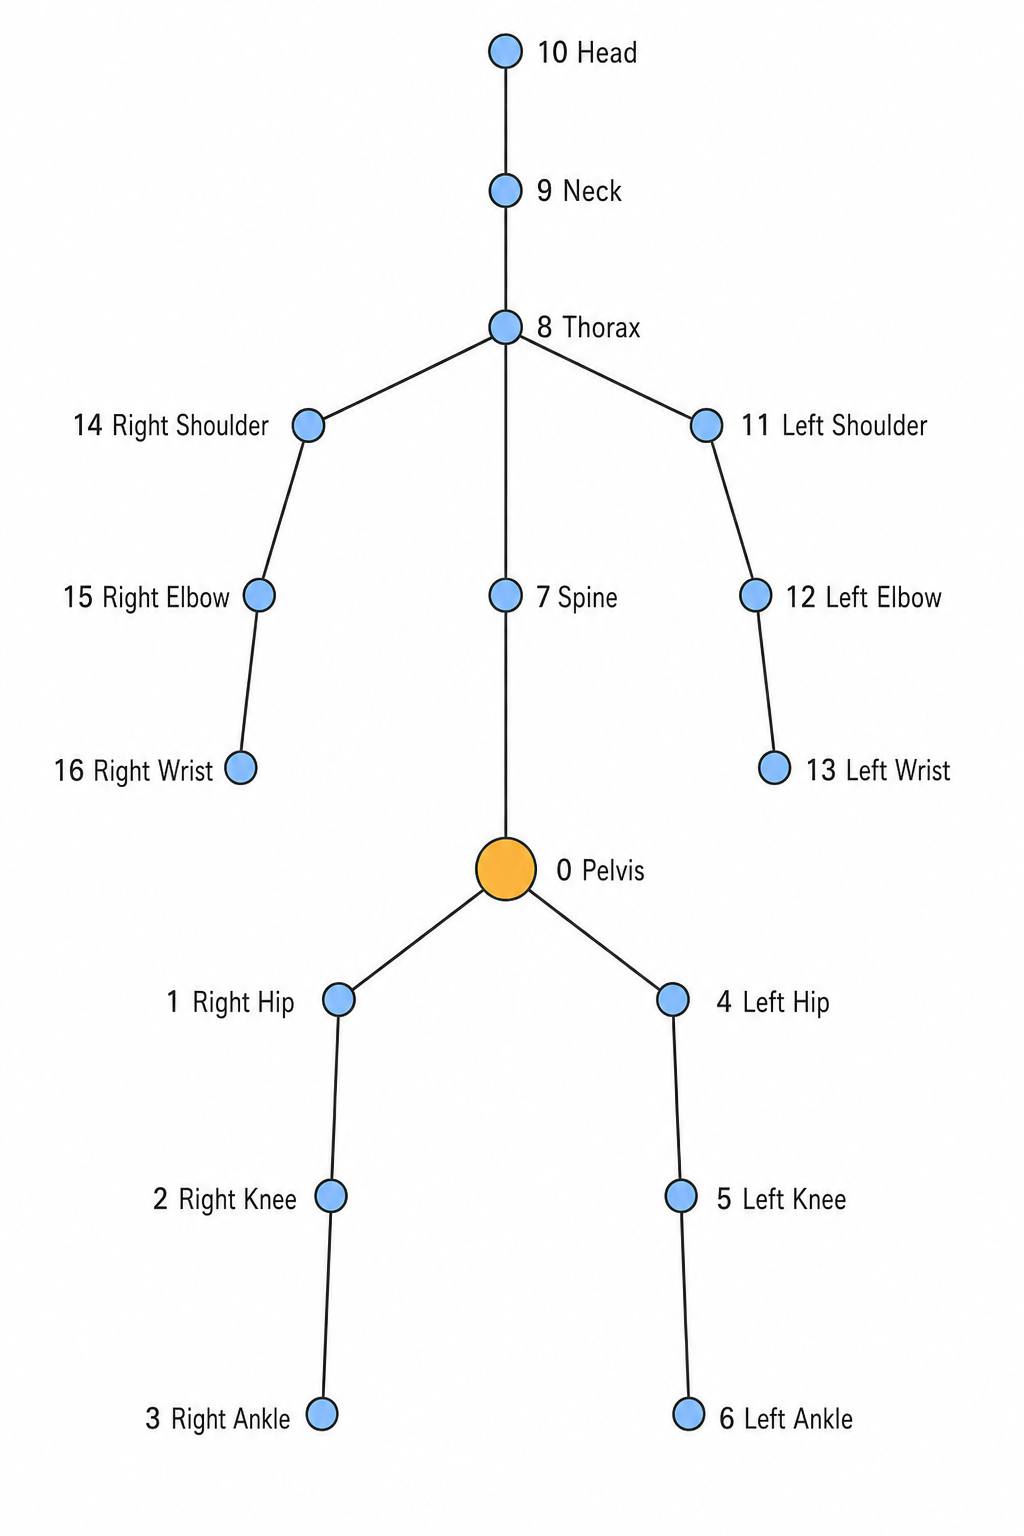
\includegraphics[width=0.85\textwidth]{figures/kinematic_tree.pdf}
\fbox{\parbox[c][6cm][c]{0.85\textwidth}{\centering\textit{[Kinematic-tree figure:
  insert \texttt{figures/kinematic\_tree.pdf}. The 17-joint Human3.6M skeleton as a
  rooted tree, pelvis (0) as root, 16 parent-child bones; each joint labelled with its
  index and name.]}}}
\caption[The Human3.6M skeleton as a rooted kinematic tree.]{The 17-joint
  Human3.6M skeleton, represented as a rooted kinematic tree $G=(V,E)$
  with the pelvis (joint 0) as root and 16 parent-child bone edges. The
  naive scan order used by default in Section~\ref{sec:method-bistssm}
  simply follows the numerical joint index shown in each node, ignoring
  this tree structure entirely.}
\label{fig:kinematic-tree}
\end{figure}

\section{Preliminaries: State Space Models}
\label{sec:method-prelim}

Before the architecture is described, this section states the state space
formulation the backbone is built on, following the line of work reviewed in
Section~\ref{sec:lit-ssm-foundations}. A continuous-time linear state space
model maps an input signal $u(t)$ to an output $y(t)$ through a hidden state
$h(t) \in \mathbb{R}^{N}$,
\begin{equation}
\dot{h}(t) = A h(t) + B u(t), \qquad y(t) = C h(t),
\label{eq:ssm-continuous}
\end{equation}
where $A \in \mathbb{R}^{N \times N}$ governs how the state evolves and $B$,
$C$ map the input in and the state out. To run on a discrete sequence, the
system is discretized with a step size $\Delta$ using a zero-order hold,
\begin{equation}
\bar{A} = \exp(\Delta A), \qquad
\bar{B} = (\Delta A)^{-1}\big(\exp(\Delta A) - I\big)\, \Delta B,
\label{eq:ssm-discretize}
\end{equation}
which turns Equation~\ref{eq:ssm-continuous} into the recurrence applied along
the sequence,
\begin{equation}
h_k = \bar{A} h_{k-1} + \bar{B} u_k, \qquad y_k = C h_k .
\label{eq:ssm-recurrence}
\end{equation}
S4 \cite{gu2021s4} made this practical at scale with a structured
parameterization of $A$, and S5 \cite{smith2022s5} recast it as a single
multi-input, multi-output system computed by a parallel scan. In all of these
the parameters $\bar{A}$, $\bar{B}$, $C$, and $\Delta$ are fixed for the whole
sequence.

Mamba \cite{gu2023mamba} makes the model \emph{selective}: it computes $B$,
$C$, and $\Delta$ as functions of the current input token, so the system can
decide at each position what to write into the state and what to read out.
This input dependence is what lets a state space model match attention on
content-dependent reasoning while keeping a recurrence that is linear in
sequence length. The resulting scan is evaluated with a hardware-aware
parallel algorithm that avoids writing the full sequence of hidden states to
slow memory. KinecMamba uses a diagonal $A$ with a hidden state of size
$N=16$, and applies this selective formulation as the core of its state space
layer (Section~\ref{sec:method-bistssm}).

\section{Architecture Overview}
\label{sec:method-architecture}

KinecMamba is a dual-stack, Mamba-based architecture that
processes the input 2D keypoint sequence in four stages: token embedding,
a stack of bidirectional spatio-temporal state space blocks, and an
output head. All internal token representations use a fixed channel width
of $C=64$.

\textbf{Token embedding.} The input $X \in \mathbb{R}^{B \times T \times J
\times 2}$ is first mapped to $C$-dimensional tokens by the Spatial Token
Embedding (STE), then augmented with temporal position information by the
Temporal Token Embedding (TTE), producing $Z^{(0)} \in \mathbb{R}^{B
\times T \times J \times C}$. Both embedding stages are detailed in
Section~\ref{sec:method-embedding}.

\textbf{Backbone.} $Z^{(0)}$ is then processed by 10 macro-stages. Each
macro-stage applies a Spatial-oriented BiSTSSMBlock followed by a
Temporal-oriented BiSTSSMBlock, for 20 BiSTSSMBlock instances in total.
Every BiSTSSMBlock, regardless of its spatial or temporal designation,
shares the identical internal residual structure detailed in
Section~\ref{sec:method-block} and is built around the same BiSTSSM layer,
a four-directional cross-scan selective state space layer (detailed in
Section~\ref{sec:method-bistssm}) operating over the full $T \times J$
grid of token embeddings. Each BiSTSSMBlock contains approximately 63,000
parameters (approximately 46,000 in the state space path and 17,000 in
the feed-forward path), giving a 20-block backbone of approximately 1.26
million parameters. The token embeddings and the linear output head add
only a small further amount, so the complete model contains on the order
of 1.26 million parameters, the figure reported for it in
Chapter~\ref{ch:results}.

\textbf{Output head.} After the final BiSTSSMBlock, the resulting
representation $Z^{(20)} \in \mathbb{R}^{B \times T \times J \times C}$ is
projected to 3D joint coordinates by an output head consisting of layer
normalization followed by a linear projection, $C \rightarrow 3$,
producing the predicted 3D pose sequence $\hat{Y} \in \mathbb{R}^{B \times
T \times J \times 3}$ defined in Section~\ref{sec:method-problem}.

In summary, the end-to-end shape flow, also shown in
Figure~\ref{fig:architecture-pipeline}, is:
\[
X \in \mathbb{R}^{B,T,J,2}
\;\xrightarrow{\text{STE, TTE}}\;
Z^{(0)} \in \mathbb{R}^{B,T,J,C}
\;\xrightarrow{\text{20} \times \text{BiSTSSMBlock}}\;
Z^{(20)} \in \mathbb{R}^{B,T,J,C}
\;\xrightarrow{\text{output head}}\;
\hat{Y} \in \mathbb{R}^{B,T,J,3}.
\]

\begin{figure}[t]
\centering
% Architecture figure: place the rendered image at figures/architecture.pdf and
% uncomment the \includegraphics line below (remove the placeholder box). The image
% is generated from figure_prompts.md (Figure 1).
% 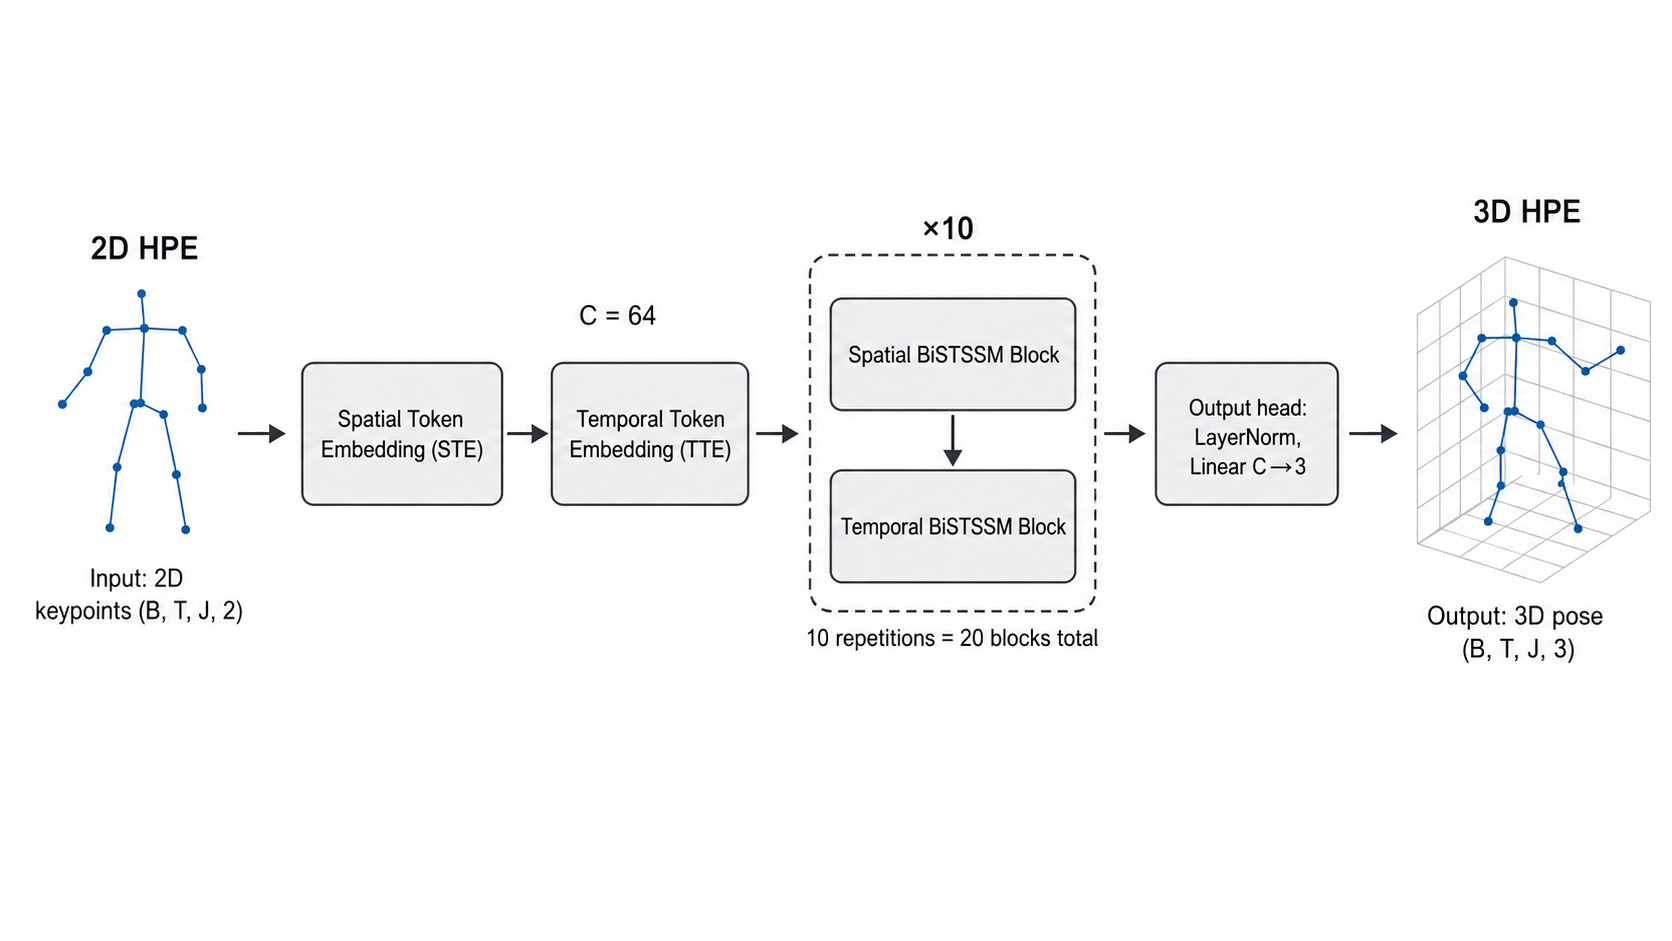
\includegraphics[width=\textwidth]{figures/architecture.pdf}
\fbox{\parbox[c][5.5cm][c]{0.92\textwidth}{\centering\textit{[Architecture
  diagram: insert \texttt{figures/architecture.pdf}. 2D-pose input
  $(B,T,J,2)$ $\rightarrow$ STE $\rightarrow$ TTE $\rightarrow$ $\times$10
  Spatial/Temporal BiSTSSM backbone (20 blocks) $\rightarrow$ output head
  (LayerNorm, Linear $C{\to}3$) $\rightarrow$ 3D-pose output $(B,T,J,3)$.]}}}
\caption[End-to-end architecture pipeline.]{End-to-end architecture
  pipeline. The input 2D keypoint sequence is embedded by the STE and TTE
  (Section~\ref{sec:method-embedding}), processed by 10 repetitions of a
  Spatial BiSTSSMBlock followed by a Temporal BiSTSSMBlock (20 blocks
  total, Section~\ref{sec:method-block}), and projected to the output 3D
  pose sequence by the output head.}
\label{fig:architecture-pipeline}
\end{figure}

\section{Spatial and Temporal Token Embedding}
\label{sec:method-embedding}

The raw input $X \in \mathbb{R}^{B \times T \times J \times 2}$ is
converted into $C$-dimensional tokens in two stages, each of which
combines a learned projection with a learned positional embedding along a
different axis.

\textbf{Spatial Token Embedding (STE).} The batch and frame dimensions are
first merged, treating every $(batch, frame)$ pair as an independent set
of $J$ joints: $X \in \mathbb{R}^{B,T,J,2} \rightarrow \mathbb{R}^{BT,J,2}$.
A shared linear layer, $\mathrm{Linear}(2 \rightarrow C)$, projects each
joint's raw 2D coordinate into the $C$-dimensional token space. A learned
spatial positional embedding $P_{\mathrm{sp}} \in \mathbb{R}^{1,J,C}$,
broadcast across the merged $BT$ dimension, is then added, so that each of
the $J$ token positions carries a fixed, learnable identity independent of
the coordinate values placed into it. The result is reshaped back to
$\mathbb{R}^{B,T,J,C}$.

\textbf{Temporal Token Embedding (TTE).} The batch and joint dimensions
are then merged instead, treating every $(batch, joint)$ pair as an
independent length-$T$ time series: $\mathbb{R}^{B,T,J,C} \rightarrow
\mathbb{R}^{BJ,T,C}$. A learned temporal positional embedding
$P_{\mathrm{te}} \in \mathbb{R}^{1,T,C}$, broadcast across the merged $BJ$
dimension, is added directly (no additional linear projection is needed
at this stage, since the tokens are already $C$-dimensional), giving each
of the $T$ frame positions a fixed, learnable identity. The result is
reshaped back to $\mathbb{R}^{B,T,J,C}$, producing $Z^{(0)}$, the input to
the first BiSTSSMBlock.

Because $P_{\mathrm{sp}}$ is indexed by joint position and added before
any scan-order permutation is applied, each token's positional identity
travels with it through any subsequent reordering of the joint axis. This
is what allows the scan order over the joint axis (the naive index order,
or the breadth-first kinematic-tree order introduced in
Section~\ref{sec:method-bfs}) to be changed without altering what
information the network has available to identify which physical joint
each token corresponds to.

\section{The Bidirectional Spatio-Temporal State Space Block}
\label{sec:method-block}

Every BiSTSSMBlock, whether spatial- or temporal-oriented, is a pre-norm
residual block containing two sub-layers: the BiSTSSM layer itself
(Section~\ref{sec:method-bistssm}) and a position-wise feed-forward
network, each wrapped in a residual connection preceded by layer
normalization. Given an input token grid $z \in \mathbb{R}^{B,T,J,C}$, the
block computes:
\begin{align}
z' &= z + \mathrm{DropPath}\big(\mathrm{BiSTSSM}(\mathrm{LayerNorm}(z))\big), \\
z'' &= z' + \mathrm{DropPath}\big(\mathrm{MLP}(\mathrm{LayerNorm}(z'))\big),
\end{align}
where $\mathrm{DropPath}$ is stochastic depth. During training, the
entire sub-layer's contribution is randomly zeroed with some probability
and the residual connection alone is passed through, which regularizes the
network without altering its structure at inference time. The
feed-forward network expands and then contracts the channel dimension,
\begin{equation}
\mathrm{MLP}(u) = \mathrm{Linear}_{128 \rightarrow 64}\big(\mathrm{GELU}(\mathrm{Linear}_{64 \rightarrow 128}(u))\big),
\end{equation}
applied identically and independently to every token in the $T \times J$
grid. This pre-norm residual design mirrors the block structure used
throughout the Transformer- and SSM-based literature reviewed in
Chapter~\ref{ch:literature-review}; what distinguishes the block proposed
here is the internal design of the BiSTSSM layer itself, detailed next.

\section{The BiSTSSM Layer: Cross-Scan Selective State Space Modeling}
\label{sec:method-bistssm}

The BiSTSSM layer is the component within each BiSTSSMBlock
(Section~\ref{sec:method-block}) responsible for modeling dependencies
across the $T \times J$ grid of token embeddings. It operates in six
steps: a four-directional cross-scan, an input projection, a depthwise
convolution, a selective state space model applied per direction, a
cross-merge, and an output projection. Figure~\ref{fig:bistssm-layer}
summarizes this pipeline.

\begin{figure}[t]
\centering
% BiSTSSM-layer figure: place the rendered image at figures/bistssm_layer.pdf and
% uncomment the \includegraphics line below (remove the placeholder box). The image is
% generated from figure_prompts.md (Figure 3, BiSTSSM layer internals).
% 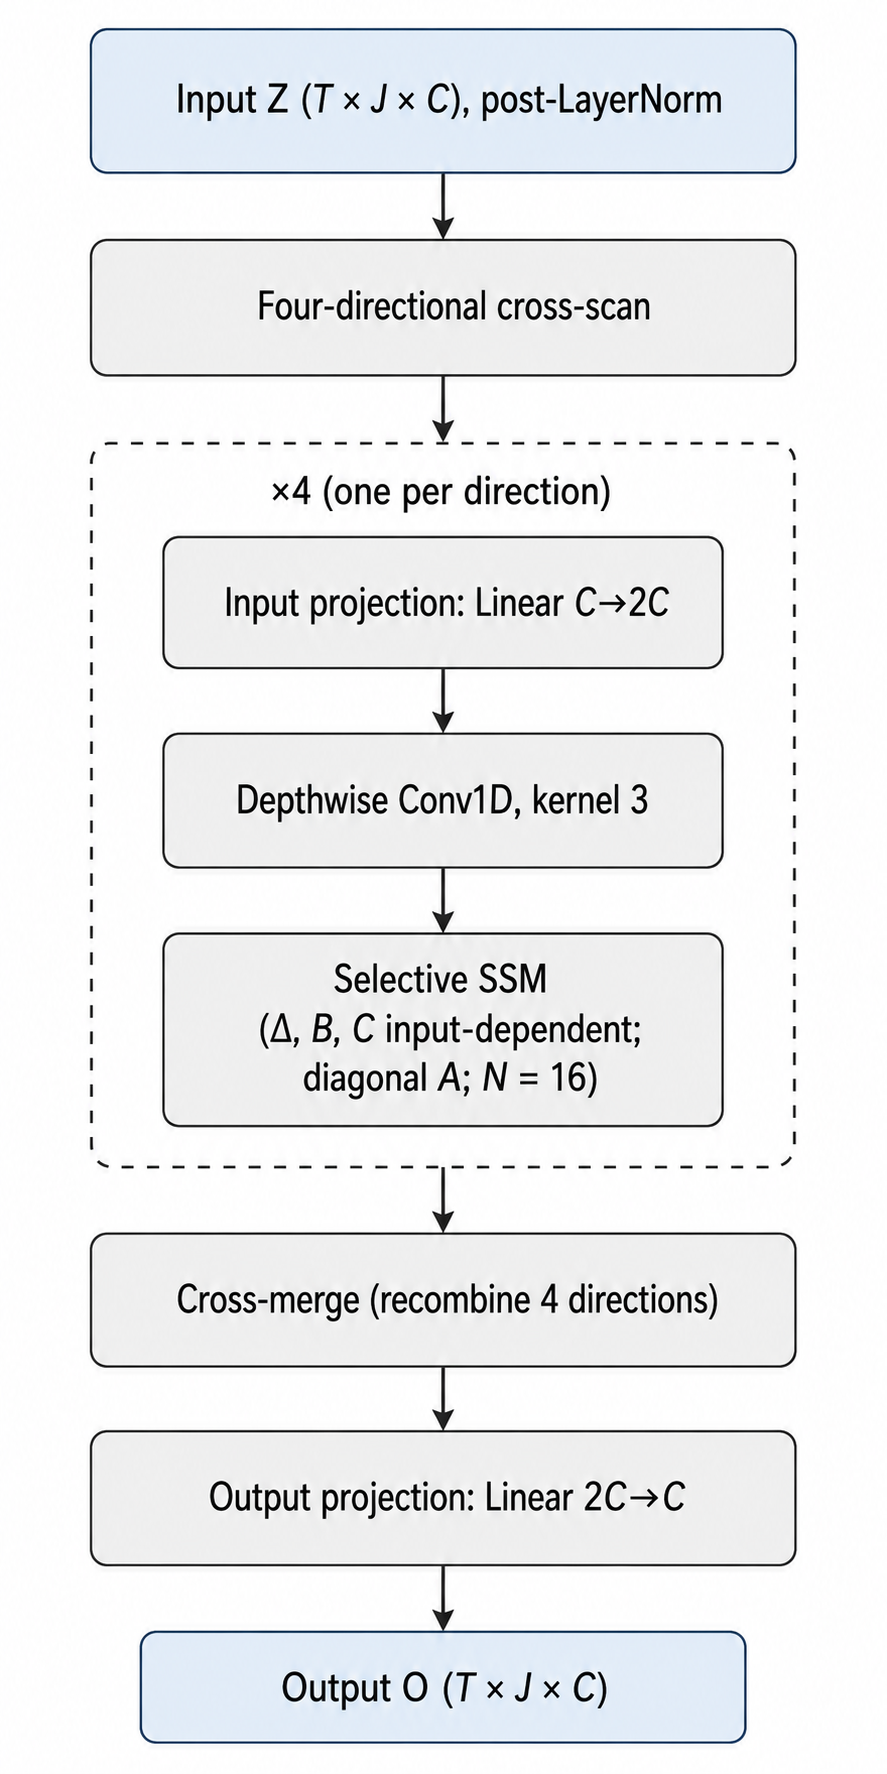
\includegraphics[width=0.6\textwidth]{figures/bistssm_layer.pdf}
\fbox{\parbox[c][6cm][c]{0.6\textwidth}{\centering\textit{[BiSTSSM-layer figure: insert
  \texttt{figures/bistssm\_layer.pdf}. Vertical pipeline: input $Z$ (post-LayerNorm)
  $\rightarrow$ four-directional cross-scan $\rightarrow$ $\times$4 (input projection
  $C{\to}2C$, depthwise Conv1D k=3, selective SSM with $N{=}16$) $\rightarrow$ cross-merge
  $\rightarrow$ output projection $2C{\to}C$ $\rightarrow$ output $O$.]}}}
\caption[The BiSTSSM layer.]{The BiSTSSM layer: the $T\times J$ token
  grid is unfolded into four directional sequences, each independently
  projected, convolved, and processed by a selective state space model,
  then recombined by the cross-merge step and projected back to the
  model's working width $C$.}
\label{fig:bistssm-layer}
\end{figure}

\textbf{Four-directional cross-scan.} A selective state space model, as
reviewed in Section~\ref{sec:lit-ssm-foundations}, processes a strictly
one-dimensional sequence, whereas the layer's input is a 2D grid of $T
\times J$ tokens. Following the cross-scan strategy introduced for
non-causal visual data by VMamba \cite{liu2024vmamba} and the
bidirectional scanning of Vision Mamba \cite{zhu2024visionmamba}, the
layer unfolds this grid into four separate 1D sequences from two natural
flattenings, each read in both directions. The first flattening is
frame-major, sweeping all joints within a frame before advancing to the next
frame; the second is joint-major, sweeping all frames for a joint before
advancing to the next joint. Reading each flattening forward and then
backward gives the four sequences. Each is processed by an independent
instance of the remaining steps below, so that every token is eventually
informed by grid neighbors reached from all four traversal directions, not
only those preceding it in a single fixed order.

\textbf{Input projection and local convolution.} Each of the four
directional sequences, with tokens of width $C=64$, is first projected to
an expanded width of $2C=128$ by a linear layer, giving the selective SSM
step below more representational capacity to work with than the model's
residual-stream width. A depthwise 1D convolution with kernel size 3 is
then applied along the sequence dimension, independently per channel,
giving each token a small amount of local context (its immediate
neighbors in the current scan order) before the global, recurrent
computation of the state space model.

\textbf{Selective state space model.} Each of the four length-$L$
sequences (where $L=TJ$) is then processed by a selective state space model,
the formulation set out in Section~\ref{sec:method-prelim}
\cite{gu2023mamba}. The post-convolution sequence supplies the input tokens
$u_k$; the hidden state has dimension $N=16$; the state matrix $A$ is diagonal
with negative entries, which keeps the recurrence stable; and $B_k$, $C_k$,
and the step size $\Delta_k$ are computed per token, so the layer decides at
each scan position what to write into and read out of the state. The
recurrence of Equation~\ref{eq:ssm-recurrence} is evaluated with the
hardware-aware parallel scan of Mamba \cite{gu2023mamba}, which never
materializes the full sequence of hidden states in slow memory.

\textbf{Cross-merge and output projection.} Once all four directional
sequences have been processed, each is reshaped back into the $T \times J$
grid layout and the four resulting grids are combined into a single
$2C$-dimensional grid representation in the cross-merge step, mirroring
the merge stage of VMamba's cross-scan \cite{liu2024vmamba}. A final linear
layer projects this merged representation from $2C=128$ back down to
$C=64$, matching the residual-stream width used by the surrounding
BiSTSSMBlock (Section~\ref{sec:method-block}).

\section{Breadth-First Search Kinematic-Tree Scan Order}
\label{sec:method-bfs}

The row-major and column-major flattenings underlying the cross-scan
described in Section~\ref{sec:method-bistssm} require an explicit order
over the $J$ joints along the spatial axis of the grid. By default, this
order is simply the joint's numerical index, $[0, 1, \ldots, 16]$, which
carries no relationship to the skeleton's actual anatomical structure: for
example, under this order, joint 3 (Right Ankle) and joint 4 (Left Hip)
are scan-adjacent despite being on opposite sides of the body and far
apart in the kinematic tree $G$ defined in
Section~\ref{sec:method-problem}. As discussed in
Section~\ref{sec:lit-skeleton-ordering}, this thesis instead orders the
joints by a breadth-first search (BFS) traversal of $G$, which visits
joints in order of their distance from the root and so keeps each joint
close in the sequence to its parent and to the other joints at its depth,
rather than to arbitrary joints elsewhere in the skeleton.

\textbf{BFS traversal.} Algorithm~\ref{alg:bfs-scan} formalizes the
traversal. Starting from the root joint (the pelvis, joint 0), the
algorithm visits joints in order of non-decreasing graph distance from the
root, breaking ties by visiting a node's children in
ascending original joint-index order. This tie-breaking rule ensures the
resulting order $\pi$ is fixed and reproducible for a given kinematic tree
$G$, in contrast to the learned Group and
Joint Scan strategies of \cite{nguyen2025skeletonmamba} reviewed in
Section~\ref{sec:lit-ssm-pose}.

\renewcommand{\algorithmicrequire}{\textbf{Input:}}
\renewcommand{\algorithmicensure}{\textbf{Output:}}
\renewcommand{\algorithmicforall}{\textbf{for each}}
\begin{algorithm}
\caption{Breadth-First Search Kinematic-Tree Scan Order}
\label{alg:bfs-scan}
\begin{algorithmic}
  \REQUIRE $G=(V,E)$: kinematic tree over joints $V=\{0,\ldots,J-1\}$
    (Section~\ref{sec:method-problem}), rooted at joint $r=0$ (pelvis)
  \ENSURE $\pi$: an ordered list of joint indices, a permutation of $V$
  \STATE $\pi \gets$ empty list; $Q \gets$ empty queue
  \STATE mark $r$ as visited; enqueue $r$ onto $Q$
  \WHILE{$Q$ is not empty}
    \STATE $v \gets$ dequeue from $Q$
    \STATE append $v$ to $\pi$
    \FORALL{children $c$ of $v$ in $E$, in ascending index order}
      \IF{$c$ is not visited}
        \STATE mark $c$ as visited; enqueue $c$ onto $Q$
      \ENDIF
    \ENDFOR
  \ENDWHILE
  \STATE \textbf{return} $\pi$
\end{algorithmic}
\end{algorithm}

Applied to the Human3.6M kinematic tree of Section~\ref{sec:method-problem},
Algorithm~\ref{alg:bfs-scan} produces the fixed order
\[
\pi = [\,0,\ 1,\ 4,\ 7,\ 2,\ 5,\ 8,\ 3,\ 6,\ 9,\ 11,\ 14,\ 10,\ 12,\ 15,\ 13,\ 16\,],
\]
that is, Pelvis; Right Hip, Left Hip, Spine; Right Knee, Left Knee, Thorax;
Right Ankle, Left Ankle, Neck, Left Shoulder, Right Shoulder; Head, Left
Elbow, Right Elbow; Left Wrist, Right Wrist. The traversal visits the
skeleton level by level outward from the pelvis, exactly as motivated in
Section~\ref{sec:lit-skeleton-ordering}. Figure~\ref{fig:scan-order-comparison}
contrasts this order directly against the naive index order it replaces:
under the naive order, anatomically distant joints (e.g.\ Right Ankle and
Left Hip) are scan-adjacent, whereas under the proposed BFS order,
scan-adjacent joints are also kinematically close.

\begin{figure}[t]
\centering
% Scan-order figure: place the rendered image at figures/scan_order.pdf and uncomment
% the \includegraphics line below (remove the placeholder box). The image is generated
% from figure_prompts.md (Figure 4, naive vs BFS scan order).
% \includegraphics[width=\textwidth]{figures/scan_order.pdf}
\fbox{\parbox[c][3.5cm][c]{0.95\textwidth}{\centering\textit{[Scan-order figure: insert
  \texttt{figures/scan\_order.pdf}. Two strips of 17 joint cells: a top ``naive index
  order'' strip (0..16) and a bottom ``BFS kinematic order'' strip
  (0,1,4,7,2,5,8,3,6,9,11,14,10,12,15,13,16), showing that the BFS order keeps
  kinematically close joints adjacent.]}}}
\caption[Naive vs.\ BFS kinematic-tree scan order.]{The 17 joints
  (abbreviated names, subscript = joint index, as defined in
  Figure~\ref{fig:kinematic-tree}) under the naive index order used by
  default (top) versus the proposed breadth-first kinematic-tree order
  $\pi$ (bottom). The BFS order visits joints level by level outward from
  the pelvis, so joints at the same depth in the kinematic tree become
  adjacent (e.g.\ the two hips and the spine root, all direct children of
  the pelvis) and every joint stays close to its parent, whereas the naive
  order interleaves joints from unrelated parts of the skeleton.}
\label{fig:scan-order-comparison}
\end{figure}

\textbf{Permute-before-scan, inverse-permute-after-merge.} Let $Z \in
\mathbb{R}^{B,T,J,C}$ be a BiSTSSMBlock's input to the BiSTSSM layer, with
joints indexed in the original order established by the spatial
positional embedding (Section~\ref{sec:method-embedding}). Before the
cross-scan of Section~\ref{sec:method-bistssm} is applied, $Z$ is reindexed
along its joint axis according to $\pi$,
\begin{equation}
Z_\pi[:,:,i,:] = Z[:,:,\pi(i),:], \qquad i = 0, \ldots, J-1,
\end{equation}
Because this reindexing is applied to the joint axis of $Z$ before either
flattening is formed, all four directional scans, in both the frame-major
and joint-major flattenings of Section~\ref{sec:method-bistssm}, traverse
joints in kinematic-tree BFS order rather than raw index order. After the selective state space model
and cross-merge produce an output $O_\pi \in \mathbb{R}^{B,T,J,C}$, still
in BFS order, the inverse permutation $\pi^{-1}$ is applied to restore the
original joint indexing,
\begin{equation}
O[:,:,\pi(i),:] = O_\pi[:,:,i,:], \qquad i = 0, \ldots, J-1,
\end{equation}
before $O$ is returned as $\mathrm{BiSTSSM}(\cdot)$ in the residual
equation of Section~\ref{sec:method-block}. This inverse permutation is
essential: without it, the residual addition $z + \mathrm{BiSTSSM}(z)$
would add each joint's input token to a \emph{different} joint's output
token, and the fixed, joint-indexed spatial positional embedding of
Section~\ref{sec:method-embedding} would no longer correspond to the
correct joint after the first block.

Because $\pi$ is derived once from the fixed kinematic tree $G$ and
applied identically to every BiSTSSMBlock, this scan order adds only a
fixed gather/scatter operation, distinguishing it from the auxiliary
topology-fusion modules and learned scan groupings reviewed in
Section~\ref{sec:lit-ssm-pose}.

\section{Computational Complexity}
\label{sec:method-complexity}

The efficiency claim behind KinecMamba can be stated directly. Let $L = TJ$
be the number of spatio-temporal tokens the BiSTSSM layer processes. The
selective state space scan of Section~\ref{sec:method-bistssm} visits each
token once and, at each step, updates a hidden state of fixed size $N$, so
its cost grows as $\mathcal{O}(L N C)$, that is, linearly in $L$ for fixed
$N$ and channel width $C$. The four directional scans and the depthwise
convolution add only constant factors. Full spatio-temporal self-attention,
by contrast, forms an $L \times L$ score matrix and therefore costs
$\mathcal{O}(L^{2} C)$, quadratic in $L$. This is the gap identified as
Problem~1 in Section~\ref{sec:intro-problem-statement}: at a sequence length
of $L = 243 \times 17 = 4131$ tokens, the quadratic term is what forces
attention-based lifters into a trade-off between temporal window and
compute, and it is what the state space backbone removes.

The breadth-first scan order does not change this analysis. It is a fixed
permutation of the $J$ joints along one axis, applied as a gather before the
scan and a scatter after the merge (Section~\ref{sec:method-bfs}), so it costs
$\mathcal{O}(J)$ per layer. KinecMamba therefore keeps the linear-time
behaviour of its backbone while changing only the order in which joints enter
the scan.

\section{Loss Function}
\label{sec:method-loss}

The network is trained with a multi-term loss. Four terms are standard in
prior 3D HPE work \cite{zhang2022mixste, zhu2023motionbert,
mehraban2024motionagformer} and target per-frame joint accuracy, robustness
to scale ambiguity, temporal velocity, and prediction smoothness. Two
further terms are anatomy-aware bone-length losses that pair with the BFS
kinematic scan of Section~\ref{sec:method-bfs}, supervising the lengths and
temporal consistency of the skeleton's bones. Let $\hat{Y}, Y \in
\mathbb{R}^{B,T,J,3}$ denote the predicted and ground-truth 3D pose sequences
defined in Section~\ref{sec:method-problem}.

\textbf{Joint position loss.} The primary supervision signal is the mean
per-joint position error (MPJPE), the mean Euclidean distance between
predicted and ground-truth joint positions:
\begin{equation}
\mathcal{L}_{3d} = \frac{1}{BTJ} \sum_{b,t,j} \big\lVert \hat{Y}_{b,t,j} - Y_{b,t,j} \big\rVert_2 .
\end{equation}

\textbf{Scale-invariant joint position loss.} Because monocular depth
estimates are subject to a global scale ambiguity, a second term evaluates
accuracy after removing any consistent scale error. For each sample, the
least-squares optimal scale factor aligning the prediction to the ground
truth,
\begin{equation}
s^{*} = \frac{\sum_{t,j} \hat{Y}_{t,j} \cdot Y_{t,j}}{\sum_{t,j} \hat{Y}_{t,j} \cdot \hat{Y}_{t,j}},
\end{equation}
is computed and applied before measuring MPJPE:
\begin{equation}
\mathcal{L}_{3d\text{-}scale} = \frac{1}{BTJ} \sum_{b,t,j} \big\lVert s^{*} \hat{Y}_{b,t,j} - Y_{b,t,j} \big\rVert_2 .
\end{equation}

\textbf{Velocity loss.} To encourage temporally coherent motion, a third
term compares frame-to-frame joint velocities of the prediction and the
ground truth, $\Delta \hat{Y}_{t} = \hat{Y}_{t+1} - \hat{Y}_{t}$ and
$\Delta Y_{t} = Y_{t+1} - Y_{t}$:
\begin{equation}
\mathcal{L}_{3d\text{-}velocity} = \frac{1}{B(T-1)J} \sum_{b,t,j} \big\lVert \Delta \hat{Y}_{b,t,j} - \Delta Y_{b,t,j} \big\rVert_2 .
\end{equation}

\textbf{Temporal smoothness loss.} A fourth term regularizes the
prediction's own frame-to-frame smoothness directly, independent of the
ground-truth velocity, via a per-joint weighted quadratic penalty on
consecutive-frame differences:
\begin{equation}
\mathcal{L}_{diff} = \frac{1}{B(T-1)J} \sum_{b,t,j} w_j \big\lVert \Delta \hat{Y}_{b,t,j} \big\rVert_2^{2},
\end{equation}
where $w_j$ is a fixed, per-joint weighting coefficient.

\textbf{Bone-length loss.} The length of each bone is fixed by the body and
should not change with pose or over time, so two anatomy-aware terms
supervise the skeleton's bones. Let $E$ be the set of 16 parent-child bones
of the kinematic tree $G$ (Section~\ref{sec:method-problem}), and let
$\ell_e(\hat{Y}_{t})$ denote the Euclidean length of bone $e$ in the
predicted pose at frame $t$. The first term matches predicted bone lengths to
the ground truth,
\begin{equation}
\mathcal{L}_{bone} = \frac{1}{BT|E|} \sum_{b,t,e} \big| \ell_e(\hat{Y}_{b,t}) - \ell_e(Y_{b,t}) \big|,
\end{equation}
and the second penalizes the temporal variance of each predicted bone length,
\begin{equation}
\mathcal{L}_{bvar} = \frac{1}{B|E|} \sum_{b,e} \mathrm{Var}_{t}\big[ \ell_e(\hat{Y}_{b,t}) \big].
\end{equation}
Both terms act on the same 16 bones the BFS scan of
Section~\ref{sec:method-bfs} traverses, so the training objective and the
scan order reinforce the same skeletal structure.

\textbf{Combined objective.} The total training loss is a weighted sum of
the six terms:
\begin{equation}
\mathcal{L} = \lambda_{3d}\, \mathcal{L}_{3d} + \lambda_{scale}\, \mathcal{L}_{3d\text{-}scale} + \lambda_{vel}\, \mathcal{L}_{3d\text{-}velocity} + \lambda_{diff}\, \mathcal{L}_{diff} + \lambda_{bone}\, \mathcal{L}_{bone} + \lambda_{bvar}\, \mathcal{L}_{bvar},
\end{equation}
with $\lambda_{3d} = 1.0$, $\lambda_{scale} = 0.5$, $\lambda_{vel} = 20.0$,
$\lambda_{diff} = 0.5$, $\lambda_{bone} = 0.5$, and $\lambda_{bvar} = 1.0$.
The comparatively large weight on $\mathcal{L}_{3d\text{-}velocity}$ reflects
its role as the primary driver of temporal consistency between predicted and
ground-truth motion, while the bone-length terms keep the predicted skeleton
anatomically consistent.

\section{Summary}
\label{sec:method-summary}

This chapter presented KinecMamba, a dual-stack, Mamba-based architecture for
monocular 3D human pose estimation. Section~\ref{sec:method-problem}
formalized the input/output representation and the skeleton's kinematic
tree, and Section~\ref{sec:method-embedding} projects the input 2D
keypoint sequence into a fixed-width token representation. A stack of 20
bidirectional spatio-temporal state space
blocks (Section~\ref{sec:method-block}), each built around a
four-directional cross-scan selective state space layer
(Section~\ref{sec:method-bistssm}), models spatial and temporal
dependencies with linear complexity in sequence length, consistent with
the efficiency motivation established in Chapter~\ref{ch:literature-review}.
The chapter's central contribution, the breadth-first search kinematic-tree
scan order (Section~\ref{sec:method-bfs}), replaces the naive joint-index
order otherwise used by this cross-scan with a traversal
derived directly from the skeleton's own parent-child hierarchy, closing
the research gap identified in Section~\ref{sec:lit-summary-gap}.
Section~\ref{sec:method-loss}
defined the loss function, which combines standard position, scale,
velocity, and smoothness terms with two anatomy-aware bone-length terms that
reinforce the same skeletal structure as the BFS scan.
Chapter~\ref{ch:results} evaluates this architecture empirically, reporting
accuracy and computational efficiency on the Human3.6M and MPI-INF-3DHP
benchmarks against the baselines identified in
Chapter~\ref{ch:literature-review}, and presenting ablation studies that
isolate the specific contribution of the BFS kinematic-tree scan order.

\FloatBarrier

